% Created 2024-07-08 Mon 22:16
% Intended LaTeX compiler: pdflatex
\documentclass[11pt]{article}
\usepackage[utf8]{inputenc}
\usepackage[T1]{fontenc}
\usepackage{ragged2e}
\usepackage{caladea}
\usepackage{graphicx}
\usepackage{longtable}
\usepackage{wrapfig}
\usepackage{rotating}
\usepackage{epigraph}
\usepackage[normalem]{ulem}
\usepackage{hyperref}
\usepackage{amsmath}
\usepackage{amssymb}
\usepackage{capt-of}
\usepackage{hyperref}
\usepackage{fancyhdr}
\title{Novena à Santa Bibiana}
 % \hypersetup{
 %  pdfauthor={},
 %  pdftitle={Novena a/à SANTO_NOME},
 %  pdfkeywords={},
 %  pdfsubject={},
 %  pdfcreator={Emacs 29.4 (Org mode 9.6.15)}, 
 %  pdflang={English}
 % }

\title{
  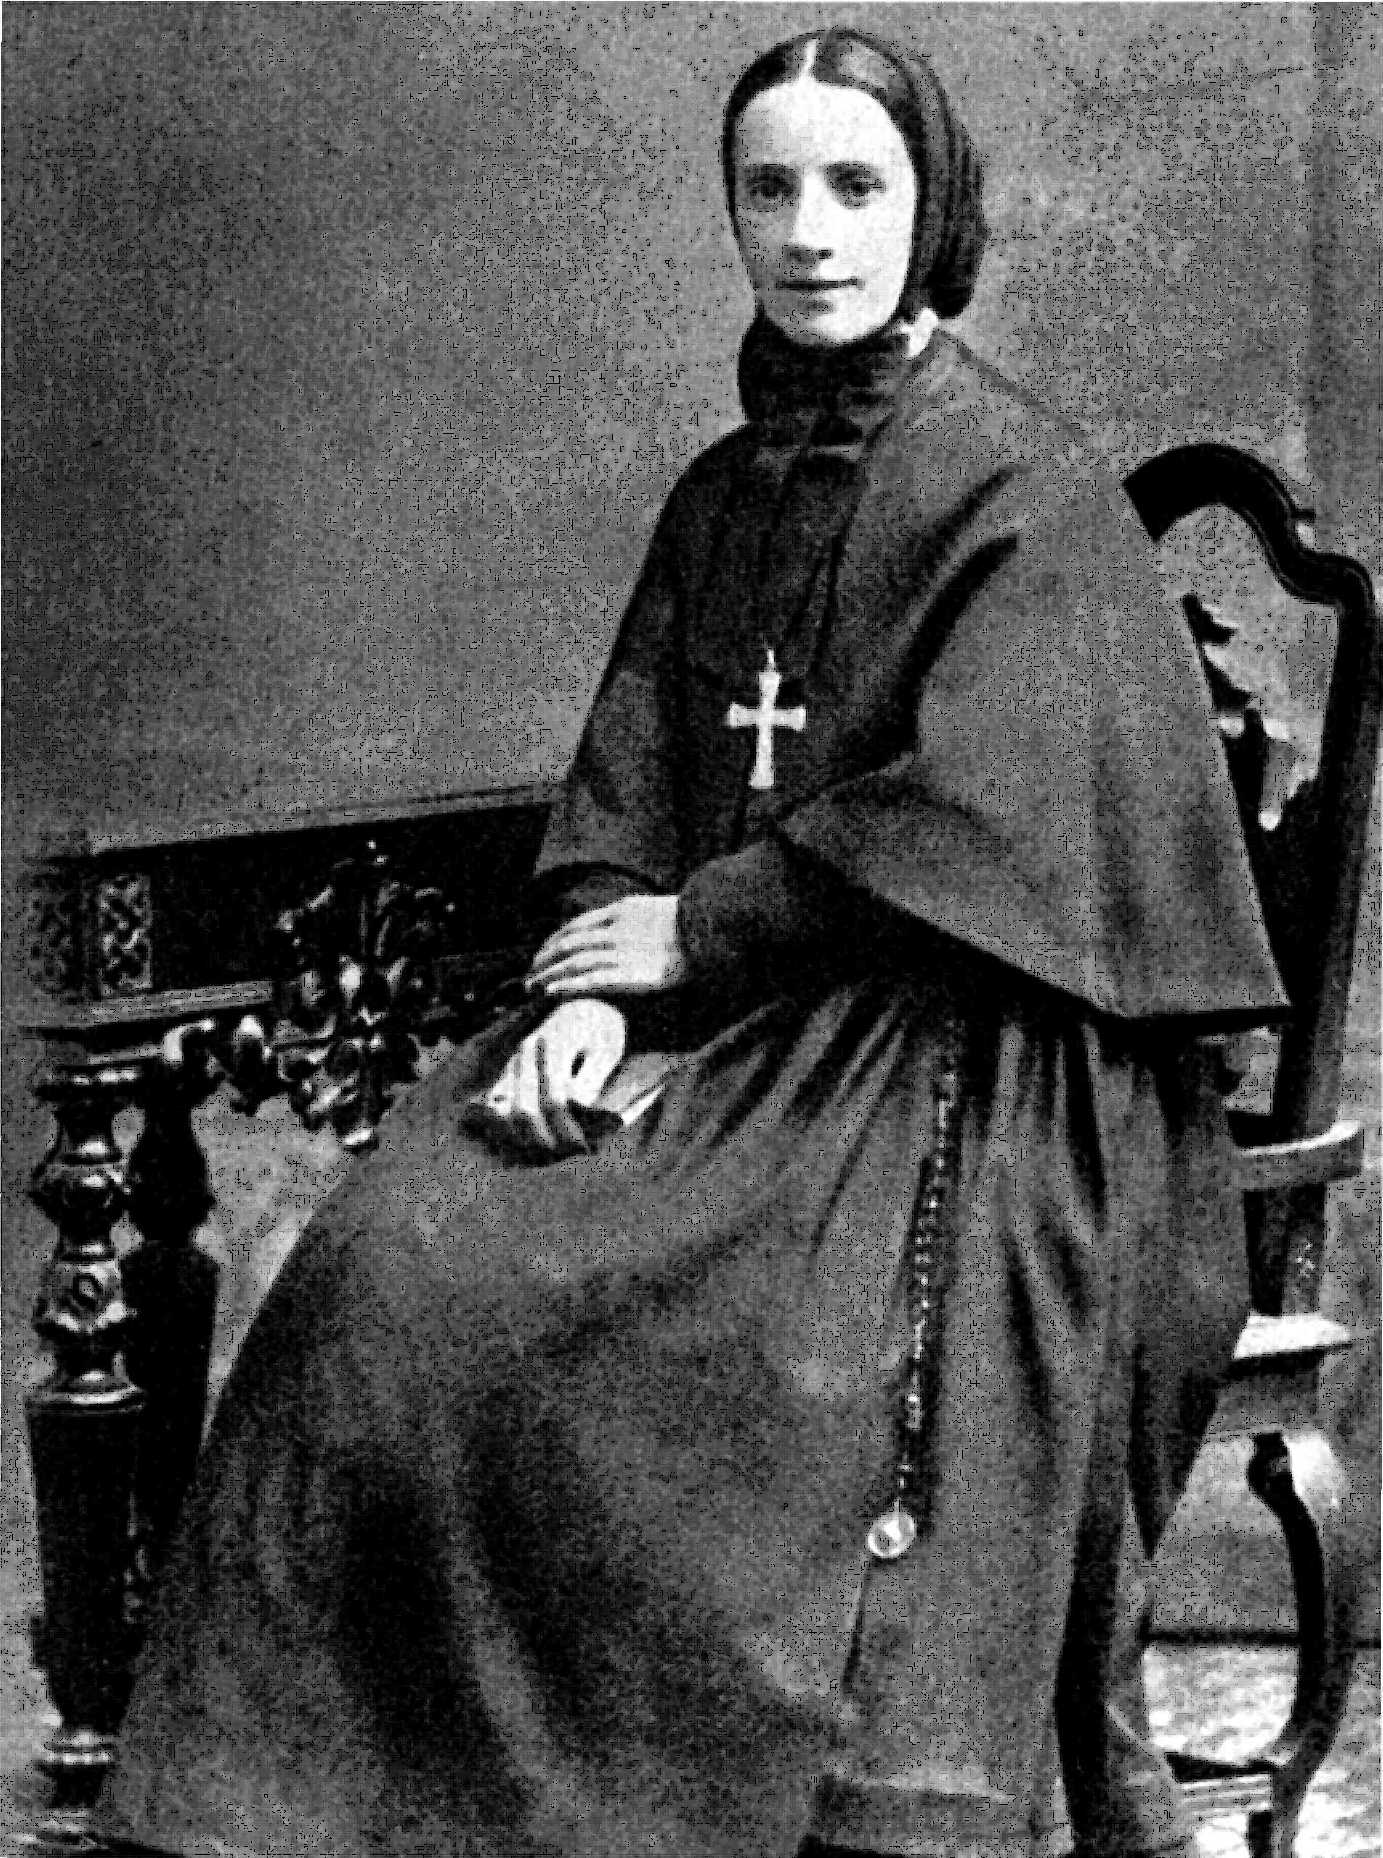
\includegraphics[scale=0.23]{./assets/imagem.jpg}
  \par
   NOVENA A SANTA FRANCISCA XAVIER CABRINI }
\author{Garamog, Nina Freitas}
\date{13/12 - 22/12}
\renewcommand{\contentsname}{Sumário}

\begin{document}


\maketitle
\thispagestyle{empty}

\pagestyle{fancy}
\fancyhf{} % clear existing header/footer entries
\fancyfoot[LO, CE]{
  
\includegraphics[scale=0.2]{./assets/cross.png} Santa Francisca Xavier Cabrini, rogai por nós!
}
% Place Page X of Y on the right-hand
% side of the footer
\fancyfoot[R]{\thepage}
  
\newpage

\tableofcontents

\centering
\vfill
Visite-nos no Telegram: \url{https://t.me/CotidieNovena}
\newpage




%%%%%%%%%%%%%%%%%%%%%%%%%%%%%%%%%%%%% História  %%%%%%%%%%%%%%%%%%%%%%%%%%%%%%%%%%%%%%%%%%%
\section{História}\label{historia}

\begin{justify}

 \hspace{.5cm}Francisca nasceu na Itália em 1850, última de uma família de 13 filhos. Ela recebe o título de “Mãe dos Imigrantes”, pois olhou para a emigração com os olhos humaníssimos de mulher, de cristã.

Nessa época, milhões de italianos emigravam para outros países, e Francisca recebeu a missão de Deus de cuidar dos interesses espirituais e materiais dessas famílias católicas que estavam no desamparo, em terras estranhas, de línguas e até religiões diferentes.

Órfã de pai e mãe queria entrar logo no convento, mas não permitiram por causa de sua idade, e sua saúde precária. Ela aceitou então o encargo de atender a um orfanato, que lhe confiou o pároco de Codogno.

Fundou a Congregação das Irmãs Missionárias do Sagrado Coração de Jesus, colocadas sob a proteção de São Francisco Xavier, de quem ela mesma pronunciando os votos, assumiu o sobrenome. Estendeu sua obra a numerosos países e cruzou o Oceano Atlântico por 30 vezes.

Faleceu aos 67 anos, em uma das viagens que fazia, em 1917. Seu corpo foi levado para Nova Iorque, para ficar perto dos emigrantes. Deixou fundadas 67 casas de sua congregação.

\end{justify}

\subsection*{Créditos }
\href{https://templariodemaria.com/santo-do-dia-22-de-dezembro-santa-francisca-xavier-cabrini/}{Templário de Maria}

\newpage


%%%%%%%%%%%%%%%%%%%%%%%%%%%%%%%%%%%%% Orações  %%%%%%%%%%%%%%%%%%%%%%%%%%%%%%%%%%%%%%%%%%%
\section{Orações}\label{oracoes}

\subsection{Oração Inicial}
Oh! Deus, vem em minha ajuda.

Oh! Senhor, apressai-vos a auxiliar-me.

\textbf{Glória ao Pai, ao filho e ao Espírito Santo. Como era no princípio, agora e sempre pelos séculos dos séculos. Amém.}\label{gloria}

Oh! Santa Francisca Xavier Cabrini, vós que obtivestes o prêmio da glória celestial por vossa vida virtuosa, ouvi a oração que confiantemente deposito em Vós e por vossos méritos, fazei que chegue até Deus e seja aceita.

\textbf{Glória ao Pai...}

Oh! Santa Francisca Xavier Cabrini, vós que durante vossa vida experimentastes amarguras e dissabores, olhai com benevolência na hora de suas necessidades a quem recorre a Vós com confiança.

\textbf{Glória ao Pai...}

Santa Francisca Xavier Cabrini, vós que com filial confiança recorreste a Onipotência Divina em todas as vossas necessidades, intercede por mim e obtém a graça que ardentemente desejo.

\textbf{Glória ao Pai...}

Oh! Santa Francisca Xavier Cabrini, vós que dissestes como o Apóstolo, "Todo o posso nAquele que me conforta", agora que vives gloriosamente com vosso Celestial Esposo implorai a graça que vos peço.

\textbf{Glória ao Pai...}

Oh! Santa Francisca Xavier Cabrini, vós que fostes enriquecida pelo Espírito Santo, com graças celestiais, obtém para mim deste Espírito Divino, que me conforte em minhas necessidades.

\textbf{Glória ao Pai...}

Oh! Santa Francisca Xavier Cabrini, vós que fostes guia e mestra de muitas almas errantes, obtém para mim também a firme crença de que alcançarás de Deus o que peças para mim.

\textbf{Glória ao Pai...}

Oh! Santa Francisca Xavier Cabrini, vós que com sumo regozijo repartiste na terra vosso auxilio como a mais terna Mãe, estende sobre mim também vossa misericórdia e proteção.

\textbf{Glória ao Pai...}

Oh! Santa Francisca Xavier Cabrini, vós que assististe aos enfermos com grande generosidade, olhai com misericórdia meus sofrimentos e obtém a graça que com confiança solicito.

\textbf{Glória ao Pai...}

Oh! Santa Francisca Xavier Cabrini, vós que através da terra derramastes o bálsamo de inextinguivel serenidade sobre o sofrimento dos corações feridos, estende a mim também vossa ajuda acolhendo a oração que devotamente deposito em vosso coração.

\textbf{Glória ao Pai...}

Roga por nós, Oh, Santa Francisca Xavier Cabrini, para que mereçamos as promessas de Nosso Senhor Jesus Cristo. Amém.

\subsection{Oração Final}
Oh! Santa Francisca Xavier Cabrini, vós que colocastes toda vossa confiança no Sagrado Coração de Jesus, e encontraste nele o segredo de toda perfeição e retidão, que vos fez uma missionária de Seu Evangelho através do mundo, pregando Sua glória no céu, olhai favoravelmente a quem com confiança recorre a vossa intercessão.

Vós que com material coração tens remediado aflições espirituais e temporais de tantos de nossos irmãos em Jesus Cristo, extraviados pelo mundo sede-me propicia em minha peregrinação durante a viagem de minha vida e obtém do Coração de Jesus todas as graças espirituais necessárias para enriquecer minha Pátria Celestial.

Oh! Santa Francisca Xavier Cabrini, ouvi minha confiante oração e obtém a graça que tão ardentemente desejo, \emph{(aqui se faz o pedido)} e concedei que eu também possa ser unido a multidão de almas que através de vossa intercessão gozam do prêmio e perdão de Deus. Amém.


\textbf{Pai-Nosso, Avé-Maria, Glória ao Pai... }

\subsection*{Créditos:}
\href{https://oracoes.info/NovenasSantas08.html}{Orações Católicas}


\end{document}
